

\newcommand{\precondQuery}[4] {
  \null %emptyline
  \subsection{#1}\label{subsec:#1}
  \begin{adjustwidth}{1em}{0pt}
    \begin{figure}[h]
      \begin{center}
        \includesvg{../images/#2}{0.65\textwidth}
        \caption{#3}
        \label{fig:#2}
      \end{center}
    \end{figure}
    #4
  \end{adjustwidth}
}

\newcommand{\sdfModel}[2] {
  \null %emptyline
  \textbf{\uppercase{#1}} 
  \begin{adjustwidth}{2.5em}{0pt}
    #2
  \end{adjustwidth}
  \null
}

\chapter{Signed Distance Field Preconditioning}\label{ch:preconditioning}

This chapter describes the adaptation of a rendering data structure, the signed
distance field, as a tool for accelerating CAD-based transport in the Direct
Accelerated Monte Carlo (DAGMC) toolkit. A model for predicting the data
structure's utilization is also introduced. Finally, demonstrations of its
effectiveness for a number of simple problems and production models are shown
and discussed.

\section{Preconditioning Theory}\label{section:preconditioner_theory}

Of the geometric queries that DAGMC supports, next surface intersection, point
containment, and closest to location are most commonly called in simulations.
At least one ray is fired to satisfy any of these queries in DAGMC with
$O(logN)$ complexity using MOAB's BVH, but it is hypothesized that these queries
can be accelerated in many cases. For each of the fundamental Monte Carlo
geometry queries in Sections \ref{subsec:Point Containment}, \ref{subsec:Next
  Surface}, and \ref{subsec:Closest Surface}, signed distance values are
recovered from the signed distance field via interploation of the field values
and used to precondition ray fire calls in DAGMC.


\precondQuery{Point Containment}
              {point_containment_sdf}
              {Examples of scenarios for point containment preconditioning using signed distance values.}
              {
                Point containment queries can be preconditioning by examining
                the interploated signed distance value for the current particle
                location. If the point's value is negative (or outside of the
                SDF), then the point is considered to be outside of the
                volume. If the point's value is positive, then the point is
                determined to be inside the volume.

                Given that there is error associated with each of these
                interpolated values, the result of this method should only be
                trusted if the absolute value of the signed distance is greater
                than the expected error associated with the value. The error If
                this is not the case, then a ray must be fired to determine the
                particle's containment with respect to the volume in
                question. In effect, this verifies that the location is far
                enough from the boundary of the volume to make a definititive
                statement about whether it is inside or outside of the volume
                based on the sign of it's interpolated signed distance value.
                Figure \ref{fig:point_containment_sdf} graphically describes the
                outcome of these different cases in 2D.
              }

\precondQuery{Next Surface}
             {next_surface_sdf}
             {Examples of scenarios for next surface intersection preconditioning using signed distance values.}
             {
               Next surface intersection queries are the most common geometry
               query in Monte Carlo simulations. The queries are intiated by
               native Monte Carlo codes to determine if a particle will cross a
               surface before reaching its next physics event location. Normally
               in DAGMC a ray is fired each time this query is called. This can
               be avoided by using the signed distance field to exclude the
               possibility of a surface crossing without explicitly determining
               the next surface intersection. If the sum of the signed distance
               values for both the current particle position and the next
               physics event location is greater than the distance between the
               two locations, then it can be guaranteed that there is no surface
               crossing along the path between those two points. The signed
               distance value represents the minimum distance to any surface for
               a given location. The signed distance value of the current
               location ensures that some portion of the particle's track from
               the current location to the physics even location is empty
               space. The signed distance value of the physics event location
               also ensures that a portion of the particle's track is empty
               space. If the entire track length can be accounted for, then no
               surface crossing exists between the two locations. Thus the
               particle can safely advance to the next physics event location
               without firing a ray. Figure \ref{fig:next_surface_sdf} depicts
               these different cases in 2D space.
               
               For robustness, the error for each interpolation should be
               subtracted from the sum of the signed distance values as a
               protective measure against invalid surface crossings. If the
               expanse between the particle's current location and its next
               physics event location cannot be accounted for by the signed
               distance values of the two points, then the next surface
               intersection will be found using a ray fire
               call. Is it acknowledged that not all
               Monte Carlo codes provide the next physics event location along
               with the particle's current location to their geometry
               kernels. In this case, preconditioning of these queries in this
               manner will not be possible.
              }

\precondQuery{Closest Surface}
             {closest_surface_sdf}
             {Examples of scenarios for closest surface preconditioning using signed distance values.}
             {
               Closest surface queries can be performed in a similar manner to
               the point containment queries, but they are more dependent on the
               native code's intent for their use. Some Monte Carlo codes always
               query for the closest surface intersection in order to
               determine whether or not the particle will exit the volume before
               reaching its next physics event location. This information can be
               interpolated from a signed distance field to the same effect.
               
               In similar fashion to the point containment case, the signed
               distance value should only be trusted if it is greater than the
               error associated with the value. Additionally, the error should
               be subtracted from the value, returning to the code a
               conservative value for the nearest intersection. If the signed
               distance value's magnitude is not greater than its error
               evaluation or if the value is negative, then a ray should be
               fired to determine the exact location of the nearest boundary
               crossing for the particle's location. Figure
               \ref{fig:closest_surface_sdf} depicts these different cases in a
               2D example.
             }
             
Using these methods, signed distance fields can act as a preconditioning tool
for the relatively expensive ray fire process to accelerated CAD-based MCRT by
using an $O(1)$ process to establish that the conditions of a geometric query
are such that a more computationally expensive ray fire is necessary before
performing the ray tracing operation. It is hypothesized that for some Monte
Carlo problems this process can be used to avoid $O(logN)$ ray fire calls to
significantly reduce the runtime of the simulation.

\section{Implementation}

\subsection{SDF Construction}

As an initial implementation, one signed distance field is generated for each
volume in DAGMC with extents matching the axis-aligned bounding box of the
volume. The signed distance field is represented as a uniform structured mesh
with a signed distance value at each vertex in the mesh as indicated in Fig.
\ref{fig:sdf_sphere}.

MOAB provides an interface for construction of structured meshes which stores
explicit vertex coordinates, hex elements, and entity handles. As with any
entity stored in MOAB, tag data can be applied to these elements. These vertex
coordinates and hex elements can be accessed using $<i,j,k>$ indexing, where the
coordinate $<0,0,0>$ and $<N_{x}, N_{y}, N_{z}>$ represent the lowest and
highest corner of the structured mesh in parameter space for a mesh containing
$N_{x},N_{y},N_{z}$ elements in the x, y, and z directions respectively. This
representation provides a fast path for verification, visualization, and proof
of concept in transport test cases for demonstration, but is relatiely memory
intensive due to the dense nature of the data structure and explicit mesh
element information stored in the database. To reduce this memory consumption,
an implicit version of the structured mesh has been implemented which takes
advantage of the uniform step size in each dimension to store only: the number
of elements in the mesh, the location of the lowest corner in that mesh, and a
flat array of the signed distance values associated with the elements of the
mesh.
%A much less memory intensive implementation in which only a box
%corner, grid step size, dimensions, and the signed distance value data are
%stored has now also been implemented.
This avoids the storage of vertex coordinates, mesh element connectivity, and
all associated handles to those entities. There is an added cost in re-computing
vertex coordinates when a signed distance value is interpolated, but this added
cost is negligible in comparison to a ray traverval and memory is of greater
concern for this spatially dense data structure. This data structure can still
interact with MOAB's structured mesh interface to generate an explicit mesh for
visualization and verification if required.

%% An initial implementation of the signed distance field employed MOAB's
%% structured mesh interface and data tagging capabilites for storage of the data
%% structure. This interface maintains a representation of the structured mesh with
%% vertex coordinates and handles at each point along with hex elements for each
%% mesh voxel. While this format is somewhat memory intensive, it provides
%% a fast path for verification, visualization, and proof of concept in transport
%% test cases for demonstration.

\begin{figure}
  \begin{center}
  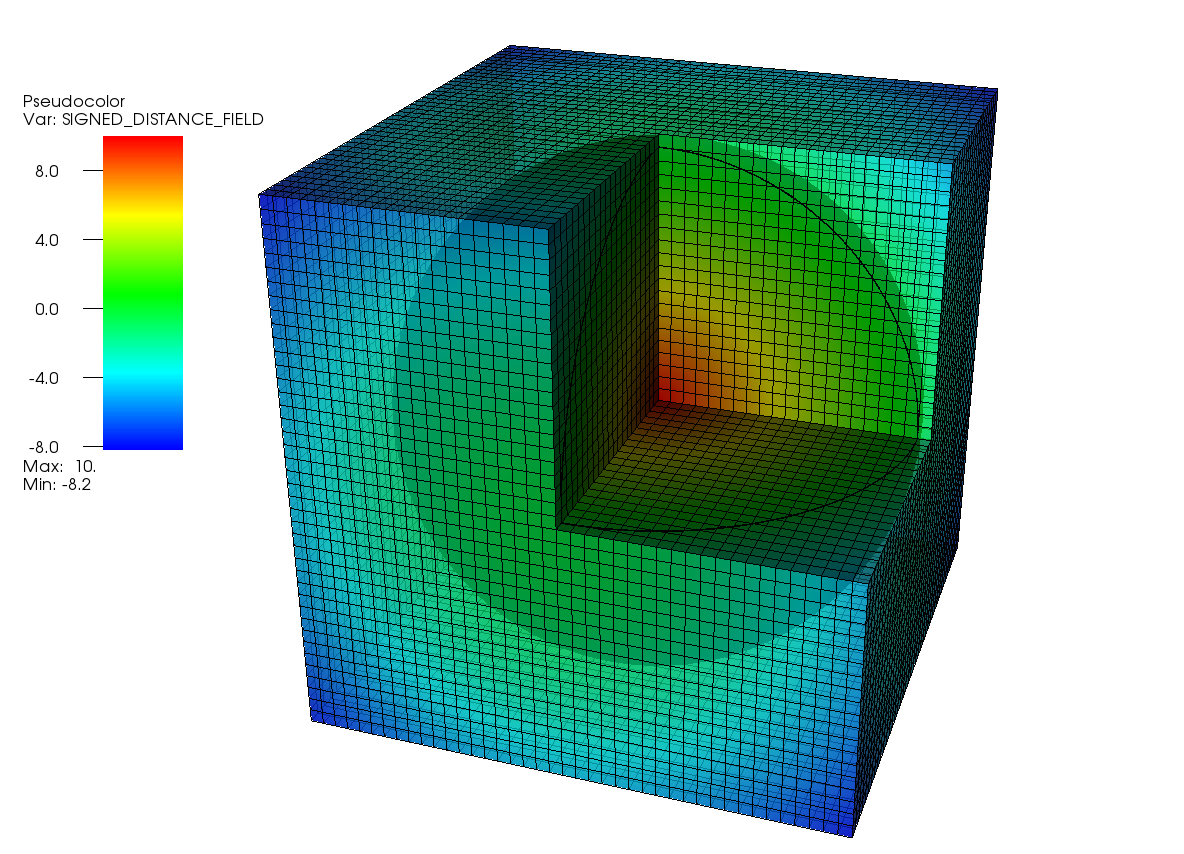
\includegraphics[scale=0.35]{../images/sdf_sphere.png}
  \caption{A visual of a signed distance field with step size 0.5 cm surrounding
    the spherical volume of test case with a radius of 10 cm.}
  \end{center}
  \label{fig:sdf_sphere}
\end{figure}

Signed distance values can be retrieved from the structured mesh by determining
which mesh voxel the point lies within. The point's element is accessed by
determining an $<i,j,k>$ index using the point's x, y, and z values divided by
the structured mesh step size. A trilinear interpolation of the mesh element's 8
vertex coordinates and their signed distance values is then used to provide the
signed distance value for the location of interest. As a result, the complexity
of a signed distance value lookup from the signed distance field is
$O(1)$.

\subsection{SDF Population}

Signed distance fields are typically generated using an implicit, analytic
representation, but a suitable data structure for populating the structured mesh
with signed distance values is already in place in the form of DAGMC's bounding
volume hierarchy. It is a more straightforward process to simply use DAGMC's
current closest to location algorithm to generate signed distance values than to
create an implicit surface approximation of the triangle mesh. This method also
maintains a consistency between the intersections found by the ray tracing
kernel and the signed distance field values.

DAGMC's closest to location algorithm returns, among other pieces of
information, the nearest intersection location and the triangle on which this
intersection exists. For each point in the signed distance field mesh, this
algorithm is used to determine the magnitude of the distance value. To
accomplish this, a ray is constructed from query location to the intersection
location. The dot product of this ray vector with the triangle's outward normal
vector is used to determine the sign of the distance value. DAGMC maintains
enough information to consistently orient triangle normals such that they point
outward from the volume they represent. In the rare cases for which the dot
product of these vectors is ambiguous, or zero, DAGMC's point containment
algorithm is used to disambiguate the value's sign.

\section{Utilization Modeling}\label{section:preconditioner_utilization}

In effect, the preconditioner is attempting to check whether or not the particle
will actually cross a surface before explicitly searching for the particle's
intersection with a surface along its current trajectory. If the result of this
preconditioning check is always false and a ray is always fired, then these
checks are only adding to the computational cost of the problem. This will
always occur in volumes filled with void, for example, as particles immediately
travel from one side of a volume to another. As a result, the signed distance field
should be applied selectively depending on each volume's geometric and material
properties for optimal performance and high utilization of the preconditioning
methods.

Ideally, this method will only be applied to volumes in which the
preconditioning method is able to avoid ray fire calls often or with high
utilization. The signed distance field is expected to have the biggest impact in
performance when preconditioning next surface intersection queries, as they are
most commonly called in Monte Carlo codes when tracking neutral particles
through the geometry (see Table . As such, this type of query is the focus of
utilization measurement for the remainder of this section.

\begin{table}[H]
  \centering
  \caption{Proportion of geom query calls for each of the simulation time calls in DAGMC.}
  \label{tab:dagmc_query_proportions}
\end{table}


\begin{equation}
  U = \frac{ \small \text{Rays Avoided w/ SDF} }{ \small \text{Number of Geometry Queries} } 
   \label{eq:preconditioner_utilization}
%  \caption{Definition of signed distance field utilization as a ray fire preconditioner in DAGMC.}
\end{equation}

As shown in Eq. \ref{eq:preconditioner_utilization}, the utilization, $U$, of
the signed distance field as a ray fire preconditioner can be described as the
number of ray fire calls related to the next surface intersection queries that
are avoided divided by the total number of next surface intersection queries
made by the Monte Carlo code. This value can be quantified using this definition
using debugging tools, such as Valgrind, to determine the number of queries made
in DAGMC and the number of rays fired inside of the subroutine.  It is expected
that in the majority of cases, as the utilization of preconditioning methods
goes up, the performance of the simulation will also improve.



\begin{figure}[ht]
  \centering
  \includesvg{../images/sdf_hydrogen_density_study_util}{\textwidth}
  \caption{Utilization results for a 5 MeV neutron source at the origin of a 10 cm radius
    sphere. Hydrogen density was varied from 0 to 1 $\frac{g}{cm^3}$.}
  \label{fig:sphere_hydrogen_density_study_util}
\end{figure}

To understand this utilization more deeply with respect to material parameters,
the hydrogen density was varied from 0 to 1 $\frac{g}{cm^3}$ in the single-volume
sphere test problem with a 5 MeV neutron point source. For each density, one
simulation was performed without the signed distance field and another with the
signed distance field and preconditioning enabled. Fig.
\ref{fig:sphere_hydrogen_density_study_util} shows the utiilzation results of this study. 

\begin{figure}[ht]
  \centering
  \includesvg{../images/sdf_hydrogen_density_study_perf}{\textwidth}
  \caption{Performance results for a 5 MeV neutron source at the origin of a 10
    cm radius sphere. Hydrogen density was varied from 0.0 to 1.0
    $\frac{g}{cm^3}$. Simulations of 100M histories at each density were
    performed using native MCNP5, DAG-MCNP5 without the signed distance field,
    and DAG-MCNP5 with the signed distance field.}
  \label{fig:sphere_hydrogen_density_study_perf}
\end{figure}

Utilization of the preconditioning method in this study remains high until the hydrogen
density falls to 0.1 $\frac{g}{cm^3}$ at which point a distinct knee appears and
the utilization falls off quickly. Even at the lowest density reached in the
study of 0.01 $\frac{g}{cm^3}$, the utilization of the signed distance field to
avoid ray fire calls is 0.54.


Fig. \ref{fig:sphere_hydrogen_density_study_perf} provides an impression of the
performance of these three implementations converge as the density of the
hydrogen is varied. As the hydrogen density approaches 1.0 $\frac{g}{cm^3}$, a
factor of ~3.5 improvement in runtime is seen in the simulation where the SDF is
applied as a preconditioner. The application of the signed distance field allows
for significantly improved performance until the density drops below 0.1
$\frac{g}{cm^3}$ in agreement with utilization plot. As the material density
decreases, particles quickly leave the geometry after very few collisions. It is
difficult to judge the impact on the performance of this simulation for these
low density values due to the limited size of the geometry and the short lived
histories.  In order to have more control over a simulation's physical
parameters, subsequent experiments were performed using a pseudo Monte Carlo
simulation tool.

\subsection{Signed Distance Field Utilization Modeling}

In order to characterize utilization of a signed distance field as a
preconditioner for next surface intersection queries in DAGMC, a pseudo Monte
Carlo simulation tool was developed using DAGMC. This tool was used to simulate
different transport scenarios within a spherical geometry with a radius of 100
cm. Particles were sourced uniformly inside the volume and scatter
isotropically. Particle histories are terminated based on a maximum number of
collisions or departure from the problem geometry. Particle distance traveled,
$d$, can be represented by either a fixed distance or by sampling for the
standard probability of interaction in a medium with mean free path,
$\lambda$. The tool allows the value of $\lambda$ to be set directly, enabling a
relation between the signed distance field and this value to be developed with
intent for use this relationship as a means for characterizing appropriate
conditions for application of the signed distance field.

\begin{figure}[H]
  \centering
  \includesvg{../images/sdf_fixed_dist_results}{\textwidth}
  \caption{Results of the model for the theoretical utilization limit with the
    results of the simulation for a fixed distance traveled case.}
  \label{fig:sdf_fixed_dist}    
\end{figure}

To begin, simulations were performed for particles with a fixed distance
traveled for varying distances and signed distance field step sizes. Run times
of the simulation are not shown here as the data structure's utilization is the
main focus of this study. The results of the study are shown in
Fig. \ref{fig:sdf_fixed_dist}. As the signed distance field mesh step size
increases, utilization of the preconditioning method structure decreases due to the increasing
error associated with the interpolation of signed distance values. Additionally,
utilization is expected to decrease with increasing distance traveled. This
decreased utilization is caused by not only the increased distance between the
two particles, but also by the increased probability that both locations will be
closer to surfaces of the sphere and have smaller signed distance values. A
theoretical limit for the utilization is also shown in
Fig. \ref{fig:sdf_fixed_dist}. The development of the analytic form for this
limit will now be discussed.

\begin{figure}[ht]
  \centering
  \includesvg{../images/alpha}{0.3\textwidth}
  \caption{Depiction of model variables.}
  \label{fig:model}
\end{figure}

\subsection{Analytic Model Development}
  
The utilization of the signed distance field as a preconditioner for ray tracing
operations can be modeled as an evaluation of the combined probability space for
particles with a current position, $\vec{p}$, and a next physics event location,
$\vec{n}$, after traveling a distance, $d$. The fraction of this probability
space in which signed distance values can be used to rule out surface crossings
for next surface intersections is then considered to be the theoretical
utilization of the signed distance field. An initial form for this probability
space can found in Eq. \ref{eq:util_model}.

\begin{equation}
  \label{eq:util_model}
\int_{V_{sphere}}\int_{V_{track}} p_p(r) p_n(d) \, \mathrm{d}V_{sphere}\mathrm{d}V_{track}
\end{equation}

In this model, the starting location of particles, $\vec{p}(r,\phi,\theta)$, is
uniformly distributed, $p_p(r)=1$, throughout a sphere of radius, $R$, centered
at the origin.  The location of the next event, $n(d,\alpha,\beta)$, where $d$
is the distance traveled by the particle, $\alpha$ is the interior angle between
the particle's \textit{position} vector and the particle's sampled direction
vector, and $\beta$ represents an azimuthal angle for directions traveled with
angle of departure, $\alpha$. Fig. \ref{fig:model} depicts these variables, $r$,
$d$, and $\alpha$ more clearly.

The outer integral in Eq. \ref{eq:util_model} represents all possible particle
positions within the geometric sphere and expands to

\begin{equation}
\int_{0}^{R}\int_{0}^{2\pi}\int_{0}^{\pi}\int_{V_{track}} r^2\sin{\phi} \, \mathrm{d}\phi
\mathrm{d}\theta \mathrm{d}r \,  p_n(d) \mathrm{d}V_{track}
\end{equation}

The inner integral over $V_{track}$ then expands to

\begin{equation}
\small \int_{0}^{R}\int_{0}^{2\pi}\int_{0}^{\pi}\int_{0}^{\infty}\int_{0}^{2\pi}\int_{0}^{\pi}
r^2\sin{\phi} \, p_n(d) d^2 \sin{\alpha} \, \mathrm{d}\alpha \mathrm{d}\beta \mathrm{d}d \, \mathrm{d}\phi
\mathrm{d}\theta \mathrm{d}r
\end{equation}

Integration of $\phi$, $\theta$, and $\beta$ can now be performed with
the knowledge that they are symmetric with respect to the problem and
integration of $p_n(d)$ does not rely on them.

\begin{equation}
\small 8\pi^2  \int_{0}^{R}\int_{0}^{\infty}\int_{0}^{\pi} p_n(d) \,
r^2 \, d^2 \sin{\alpha} \, \mathrm{d}\alpha \mathrm{d}d \, \mathrm{d}r
\end{equation}

In order to represent particles traveling a fixed distance, the relationship in Eq. \ref{eq:pn_fixed}
is applied.

\begin{equation}
  \label{eq:pn_fixed}
  p_n(d) = \frac{\delta(d-\lambda)}{d^{2}}
\end{equation}

The evaluation of this integral then gives a representation of all the query
space available to the problem

\begin{equation}
  \label{eq:A_fixed}
\small A = 8\pi^2  \int_{0}^{R}\int_{0}^{\infty}\int_{0}^{\pi} \delta(d-\lambda) \,
r^2 \, \sin{\alpha} \, \mathrm{d}\alpha \mathrm{d}d \, \mathrm{d}r
\end{equation}

and represents all geometric query space, labeled $A$, for a sphere of radius,
$R$ and a fixed distance traveled, $\lambda$.

In order to understand what fraction of this query space is able to be
preconditioned, the condition for avoiding an explicit nearest intersection
search along a particle direction in Eq. \ref{eq:condition} will now be
applied.

\begin{equation}
  SDV(\vec{p}) + SDV(\vec{n}) > |\vec{p}-\vec{n}| + 2\varepsilon(h)
  \label{eq:condition}
\end{equation}
\begin{align*}
 &SDV - \, signed \, distance \, value \, function \\
 &\vec{p} - \, particle's \, current \, position \\
 &\vec{n} - \, particle's \, next \, event \, location \\
 &h - \, mesh \, step \, size \\
 &\varepsilon(h) - \, error \, evaluation \, for \, signed \, distance \, values \\
\end{align*}

This condition establishes that the nearest location to intersection for both
points must be greater than the distance between the two points plus any error
associated with their signed distance values as previously discussed. This
condition is true for some fraction of the next surface queries in a Monte Carlo
simulation, but not all.  This model does not account for error, making it an
idealized model representing the largest utilization possible for any given
pseudo simulation.

\begin{equation}
SDV(\vec{x}) =  R-|\vec{x}|
\end{equation}

Making these substitutions into the inequality gives

\begin{equation}
R-|\vec{p}| + R - |\vec{n}| >   |\vec{p}-\vec{n}|
\end{equation}
The right hand side of this inequality can be described as the distance
traveled, $d$, and the magnitude of $\vec{p}$ can be represented
by the variable $r$.

\begin{equation}
 R-r + R - |n(d,\alpha,\beta)| > d
\end{equation}

Reducing the next event location, $\vec{n}(d,\alpha,\beta)$, into an expression
in terms of $r$, $d$, and $\alpha$ requires further examination of the
problem. Because the coordinates of $n$ depend on the current particle position,
the magnitude of $n$ with respect to the geometry origin must be obtained to get
a correct form for the signed distance value. Again, Fig. \ref{fig:model} depicts the
value of $n$ graphically for reference. The magnitude of n can then be described
using the law of cosines as

\begin{equation}
|n(d,\alpha,\beta)| = \sqrt{r^2 + d^2 - 2rd \cos{\pi-\alpha}}
\end{equation}
inserting this into the inequality gives

\begin{equation}
R-r + R - \sqrt{r^2 + d^2 + 2rd \cos{\alpha}} > d
\end{equation}

The inequality has now been reduced to the three variables seen in
Eq. \ref{eq:A_fixed}:$r$, $d$, and $\alpha$. This inequality can be applied to
construct limits of integration representing boundaries of space in which the
SDF can be utilized. By rearranging the inequality, a limit on the angle of
departure, $\alpha$, from the particle's position can be derived.

\begin{equation}
\alpha_{min} > \arccos\Bigg ( \frac{(2R-r-d)^2-d^2-r^2}{2 d r} \Bigg )
\end{equation}

\begin{figure*}[ht]
  \centering
  \includesvg{../images/model_cases_fixed_distance}{\textwidth}
  \caption{Depiction of modeling cases. Left: an example of a track for which
    $d < R - r$. Middle: an example of a track for which $R-r < d < R$ and can be
    preconditioned.  Right: an example of a track for which $R-r < d < R$ and
    cannot be preconditioned.}
  \label{fig:modeling_cases}
\end{figure*}

This condition on alpha can be interpreted as a minimum interior angle that the
particle's trajectory must take relative to the particle's position vector,
$\vec{p}$, for a distance traveled, $d$, for a ray fire to be avoided and the
preconditioner to be utilized. The examination of this condition as a function
of the distance traveled for various values of $r$ results in some conclusions
about how signed distance values are being utilized.

The inequality is undefined until the distance reaches a value $d = R- r$. This
is because the angular limit only needs to be applied to areas of the query
space in which the distance traveled is large enough to violate the above
condition as depicted in Fig. \ref{fig:modeling_cases}. A violation of this
limit may only occur when a particle travels far enough to reach the geometric
sphere boundary along the current position vector as if it were moving directly
toward the boundary of the sphere. An additional interesting feature of Figure
\ref{fig:alpha_min} is the convergence of all the curves on $\pi$ as $d$
approaches $R$. The convergence on $\pi$ indicates that as the distance traveled
approaches $R$ the only direction that the particle can move is back toward the
origin along the position vector. It also defines a maximum distance a particle
can travel in the sphere and still be preconditioned using signed distance
values. Intuitively this makes sense as the maximum chord length of a sphere is
$2R$, and once a particle travels a distance $R$ the sum of the signed distance
values can then be no larger than $R$ and the condition for utilization in
Eq. \ref{eq:condition} is violated. Hence all curves go to zero at $\lambda =
100 cm$ in Fig. \ref{fig:sdf_fixed_dist}.

In order to account for the fact that the form of $\alpha_{min}$ is undefined
until $d = R-r$, a Heaviside function is applied before applying it as a limit
on the particle's angle of departure from the position vector. Similarly,
because the $\alpha_{min}$ condition is undefined after $d=R$ a Heaviside
function is used to limit the condition to $\pi$ for any distances traveled
larger than $R$.

\begin{equation}
  \small
  \begin{split}
  \alpha_{min} =& (H(d-(R-r))-H(d-R)) \arccos\Bigg ( \frac{(2R-r-d)^2-d^2-r^2}{2 d r} \Bigg ) \\
  &+ \pi \, H(d-R)
  \end{split}
\end{equation}


By inserting this condition as a lower limit of the $d\alpha$ integration,
Eq. \ref{eq:subs_a_cond} will give all utilized space, $US$, in the query space
of the simulation.

\begin{equation}
\small US = 8\pi^2  \int_{0}^{R}\int_{0}^{\infty}\int_{\boldsymbol{\alpha_{min}}}^{\pi} \delta(d-\lambda) \,
r^2 \, d^2 \sin{\alpha} \, \mathrm{d}\alpha \mathrm{d}d \, \mathrm{d}r
\label{eq:subs_a_cond}
\end{equation}

Evaluating this integral and dividing by all query space gives the
following form for the theoretical limit of signed distance field utilization as a
preconditioner for ray firing

\begin{equation}
U_{theoretical} = \frac{US}{A} =  \frac{(1-H(\lambda-R))(2R-\lambda)(R-\lambda)}{2R^2}
\end{equation}

It can be seen in Fig. \ref{fig:sdf_fixed_dist} that this utilization limit
works well as an upper limit for the simulation results using various signed
distance field mesh resolutions. As the step size of the mesh approaches zero,
so does the evaluation of the error, resulting in the same utilization curve
with varying distance traveled, $\lambda$, as in the analytic form developed
here. Future work will include the comparison of this utilization limit to other
single-volume geometries using dimensionless parameters to determine if the
model above can be used to predict signed distance field utilization in other
geometries as well.

%% After the agreement of the simulation results and analytic model for signed
%% distance field utilization for the fixed distance traveled case, the simulation
%% was used to produce a similar set of results in which the distance is
%% sampled based on the standard probability for distance to interaction in a
%% medium with a cross section, $\Sigma$, or mean free path $\lambda
%% =1/\Sigma$. This results in the probability distribution function shown in
%% Eq. \ref{eq:pn_sampled} for the particle distance traveled in this scenario.

%% \begin{equation}
%%   \label{eq:pn_sampled}
%% p_n(d) \propto \frac{e^{-\Sigma d}}{d^{2}} = \frac{e^{-\frac{d}{\lambda}}}{d^{2}}
%% \end{equation}

%% \begin{figure}[ht]
%% \centering
%% \includesvg{../images/sdf_sampled_dist_results}{0.5\textwidth}
%% \caption{Results of the model for the theoretical utilization limit with the
%% results of the simulation for a sampled distance traveled case.}
%% \label{fig:sdf_sampled_dist}
%% \end{figure}

%% %has to be in this section for latex reasons. grumble grumble...
%% \begin{table*}[!h]
%%   \centering
%%   \begin{tabular}{lcccc}
%%           \multicolumn{5}{l}{\textbf{\textit{Source Location:}} <0,0,-1>} \\
%%           \textbf{Implementation} & \textbf{ctme (min)} & \textbf{wall time
%%             (min)} & \textbf{time ratio} & \textbf{precond. utilization}\\
%%           \hline
%%           MCNP6 & 0.17 & 0.14 & 1 & N/A \\
%%           DAG-MCNP6 & 1841.33 & 1841.33 & ~11,000 & N/A \\
%%           DAG-MCNP6 w/ SDF & 0.48 & 0.46 & 2.82 & 0.94\\
%%           \multicolumn{5}{l}{} \\
%%           \multicolumn{5}{l}{\textbf{\textit{Source Location:}} <0,0,10>} \\
%%           \textbf{Implementation} & \textbf{ctme (min)} & \textbf{wall time
%%             (min)} & \textbf{time ratio} & \textbf{precond. utilization}\\
%%           \hline
%%           MCNP6 & 0.18 & 0.18 & 1 & N/A \\
%%           DAG-MCNP6 & 11.12 & 11.16 & 62 & N/A \\
%%           DAG-MCNP6 w/ SDF & 0.50 & 0.52 & 2.89 & 0.96 \\
          
%%   \end{tabular}
%%   \caption{Performance results for an MCNP6 test case involving electron
%%     transport of a 1 keV-100 keV photon source incident on an Fe/W target. 5,000
%%     histories were run in this test problem.}
%%   \label{tab:inp066_results}
%% \end{table*}

%% Following the same process as in the fixed distance case by plugging Eq. \ref{eq:pn_sampled} into
%% Eq. \ref{eq:subs_a_cond}, the utilization form for the sampled distance case is
%% shown in Eq. \ref{eq:sampled_limit}.

%% \begin{equation}
%%   \label{eq:sampled_limit}
%%   U_{theoretical} = \frac{US}{A} = \frac{ \frac{1}{2} \lambda(R - 2 \lambda) e^{\frac{-R}{\lambda}} + \lambda^2 - \frac{3}{2} R \lambda + R^2 }{R^2}
%% \end{equation}

%% The results of this set of simulations can be seen in
%% Fig. \ref{fig:sdf_sampled_dist}. In this scenario, it is not expected that the
%% utilization will approach zero when $\lambda = 100\, cm$, as the actual distance
%% sampled may be considerably less than the provided mean free path for the
%% simulation. Overall utilization values in this scenario for $\lambda$ from 0 to
%% 100 cm remain higher than the corresponding fixed distance simulation cases as
%% is expected in a sampled distance case. Utilization values remain high for
%% relatively large increases in mesh step size, $h$. This is important to
%% application of the data structure given concerns regarding its potentially high
%% memory footprint for large volumes. For example if the utilization of the signed
%% distance field drops $~20\%$ when going from a step size of 1 cm to 6.21 cm, but
%% the memory footprint of the data structure will have decreased by a factor of
%% $6.21^3$ or $239.5$ as well. The optimization of the mesh step size with respect
%% to its effect on utilization will also need to be included in future models of
%% the utilization.


The fixed distance traveled scenario provides a nice baseline for agreement
between the computational results and the model, but a more realistic scenario
is required before attempting to apply the model as a predicitive utility for
application of the SDF in true Monte Carlo codes. The most useful alteration of
the current simulation scenario is to move from a fixed distance distance to a
sampled distance based on the standard probability for distance to interaction
in a medium given a cross section, $\Sigma$.

$$ p = e^{-\Sigma d} = e^{-\frac{d}{\lambda}} $$

where in this case now $\lambda$ represents the mean free path of the particle in the medium

In simulation, distances are now sampled as

$$ d = -\lambda ln(p) $$

where p is randomly sampled with a uniform distribution between 0 and 1

Inserting this definition for the particle distance into the integrals above
gives

$$ \frac{dp}{dd} = -\frac{p}{\lambda} $$
$$ d = 0 \rightarrow p = 1 $$
$$ d = D \rightarrow p = 0 $$

$$ \int_{0}^{R}\int_{0}^{2\pi}\int_{0}^{\pi}\int_{1}^{0}\int_{0}^{2\pi}\int_{0}^{\pi}
-r^2\sin{\phi} \, \lambda p ln(p)^2 \sin{\alpha} \, \mathrm{d}\alpha \mathrm{d}\beta \mathrm{d}p \, \mathrm{d}\phi
\mathrm{d}\theta \mathrm{d}r $$

This integral can then be evaluated to give the entirety of the geometry space
for the problem

\begin{center}
All Query Space = $\frac{4}{3} \lambda \pi^2 R^3$
\end{center}

To find the portion of utilized space for a given $R$ and $\lambda$ one can
apply the same methods from the fixed distance case, for each particle position
within the sphere there will still be two scenarios - one in which the distance
traveled exceeds $R-d$ and another in which it is less than $R-d$. The difference
now is d has become a distrubution rather than a constanct value, so as the
distance traveled changes the queries will fall into either category for a
single particle position.

Another way of viewing of viewing this condition in the case of a varying
distance is to define these same categories based on the distance traveled. Now
rather than defining how the angular condition is applied based on position, the
angular condition will be applied based on the distance the particle travels.

$$ d < R-r : \alpha_{min} = 0 $$
$$ d > R-r : \alpha_{min} = \arccos\Bigg ( \frac{(2R-r-d)^2-d^2-r^2}{2 d r} \Bigg
) $$

It is interesting to examine plots of the angular limit with varying distance as
seen in Fig. \label{fig:alpha_min}

\begin{figure}[ht] \label{fig:alpha_min}
\centering
\includesvg{alpha_r}{1\textwidth}
\caption{Plot of mininum angle of departure restriction for particles with
various radial positions and distances traveled.}
\end{figure}

The entry point of each curve in the plot represents the minimum distance
necessary to enter the $d > R-r$ region and begins to apply an agular
restriction. Note that each of these approach a mininmum angle of $\pi$ as the
distance traveled approaches $R$ (100cm). This represents a particle traveling
back towrd the origin along the sphere's larges chord with length $2R$ and,
again,the maximum distance a particle can travel before the SDF can no longer be
utilized.

Now that the distance traveled is being used to construct these two regions in
the model, this integral must be separated into two pieces, one with limits of $0$
to $R-r$ and another with limits $R-r$ to $R$. Based on the distance sampling
distribution, these values become

$$ d_{min} = R-r \rightarrow p_{max} = e^{(-\frac{(R-r)}{\lambda})} $$
$$ d_{max} = R   \rightarrow p_{min} = e^{(-\frac{R}{\lambda})} $$

and our integral becomes

$$ \int_{0}^{R}\int_{0}^{2\pi}\int_{0}^{\pi}\int_{1}^{p_{max}}\int_{0}^{2\pi}\int_{0}^{\pi}
-r^2sin(\phi) \, \lambda p ln(p)^2 sin(\alpha) \, \mathrm{d}\alpha \mathrm{d}\beta \mathrm{d}p \, \mathrm{d}\phi
\mathrm{d}\theta \mathrm{d}r + $$
$$ \int_{0}^{R}\int_{0}^{2\pi}\int_{0}^{\pi}\int_{p_{max}}^{p_{min}}\int_{0}^{2\pi}\int_{alpha_{min}}^{\pi}
-r^2\sin{\phi} \, \lambda p ln(p)^2 \sin{\alpha} \, \mathrm{d}\alpha \mathrm{d}\beta \mathrm{d}p \, \mathrm{d}\phi
\mathrm{d}\theta \mathrm{d}r $$

The evaluation of this integral divided by the full geometry query space for the
distance sampling scenario after the $c=\frac{R}{\lambda}$ replacement is

\begin{align*}
  U(c) = &\frac{1}{4c^{2}} \Big{[} (4 c^2-6) c^2e^{-2c} - (c^3-c^2-\frac{3}{2} c+3)4ce^{-2c} \\
    &+ (-2 c^3+2c^2+9c-6) e^{-2c}+4c^2-9 c+6 \Big{]}
\end{align*}

\begin{figure}[ht] 
\centering
\includesvg{../images/sdf_sampled_dist_results}{\textwidth}
\caption{Results of the model for the theoretical utilization limit with the
  results of the simulation for a fixed distance traveled case.}
\label{fig:sdf_sampled_dist}
\end{figure}

Unfortunately the predictive model for the sampled distance scenario is not
consistent with the simulation results, and under predicts the utilization of
the SDF significantly. It is quite possible that utilization in either th interior or exterior
resion of the sphere is being under represented. Regardless of the cause, examining the contribution to
utilization from each of these regions (shown in
Fig. \label{fig:util_region_contributions}) is an interesting endeavor.


\begin{figure}[ht] 
\centering
\includesvg{../images/util_contributions}{\textwidth}
\caption{A plot of the total predicted utilization along with the contriubtions
  from the inner region ($d < R-r$) and outer region ($d > R-r$).}
\label{fig:util_region_contributions}
\end{figure}

Figure \ref{fig:util_region_contributions} depicts the utilization of the SDF
data structure for various values of the mean free path, $\lambda$.
When $\lambda$ is very small, particles' next event locations
rarely reach the outer region condition of $ d > R - r $. As $\lambda$ increases, particles are
more likely to enter that region and its contribution increases greatly. Then
as particles begin to travel distances on the order of the sphere radius the
utilization decreases. The interior region utilization acts as one would
expect. When particles travel small distances with respect to the sphere radius,
there is high utilization, but as the particles begin to travel further its
utilization rapidly decreases. The contribution from the outer region defines the
significance of using both the current position signed distance value as well as the
next event location's signed distance value to precondition ray fire calls in DAGMC.

\subsection{Applying SDF Error Evaluation}

Thus far, the error associated with the tri-linear interpolation used to recover
signed distance values from the signed distance field has been ignored. In
order to optimize step size of the uniform mesh making up the signed distance
field, it is important to take this error into account when predicting the
utilization of the data structure.

As seen in Figure \ref{fig:sdf_sampled_dist}, the step size of the mesh can
significantly impact the utilization of the data structure and in turn the
overall performance of the simulation. It is important to use a step size which
will not artificially limit the effect of the data structure, but the signed
distance field is a dense data structure and uses a considerable amount of
memory. The memory usage of the signed distance field is inversely proportional
to the cube of the mesh step size ($\alpha \frac{1}{h^{3}}$). Therefore it is
important to consider the impact that this error will have on the utilization
of the data structure.

The expansion of Eq. \ref{eq:condition} with the error term maintained results in
a new condition for the minimum angle of departure ($\alpha_{min}$) shown in
Eq. \ref{eq:min_alpha_w_error}

\begin{equation}
\small
\begin{split}
\alpha_{min} =& \arccos\Bigg ( \frac{(2R-r-d-2\epsilon)^2-d^2-r^2}{2 d r} \Bigg )[H(d-(R-r-\epsilon))-H(d-(R-\epsilon))]  \\
&+ \pi \, H(d-(R-\epsilon))
\end{split}
\label{eq:min_alpha_w_error}
\end{equation}

This formulation of $\alpha_{min}$ can be used directly in the integration described
in Eq. \ref{eq:subs_a_cond}. The final form of the model after the integration being:

$$ US_{sampled} = \frac{(R-\epsilon) (\frac{1}{2} \lambda ( R - 2\lambda - \epsilon ) e^{\frac{-R + \epsilon}{\lambda}} +
\lambda^{2} - \frac{3}{2}\lambda(R - \epsilon) + (R-\epsilon)^{2})}{R^3}$$


%% For a direct evaluation of the utilization based on
%% the mesh step size, $h$, the formula for the error can be substituted for
%% $\epsilon$ to give

%% \begin{equation}
%% \small
%% \begin{split}
%% \alpha_{min} =& (H(d-(R-r-\sqrt{3}h))-H(d-(R-\sqrt{3}h))) \arccos\Bigg ( \frac{(2R-r-d-2\sqrt{3}h)^2-d^2-r^2}{2 d r} \Bigg ) \\
%% &+ \pi \, H(d-(R-\sqrt{3}h))
%% \end{split}
%% \end{equation}

This updated model was then compared to pseudo-simulations using sampled
distances for the next physics event location. The result of this can be seen in
Figure \ref{fig:sdf_util_sampled_distance_w_error}.

\begin{figure}[ht]
  \centering
  \includesvg{../images/sdf_util_sampled_distance_w_error}{\textwidth}
  \caption{Theoretical limits for SDF utilization accounting for error
    evaluation plotted with simulation results for varying mesh step sizes.}
  \label{fig:sdf_util_sampled_distance_w_error}
\end{figure}

\subsection{Extension to other geometries}

To apply this model to other geometries, the mean free path and mesh step size
were normalized using a measure of the free space in a volume compared to its
surface area, the average chord length ($R_av$) \cite{Wigner_1981}.  This value
can be defined as seen in Eq. \ref{eq:average_chord_length}.

\begin{equation}
\centering
 R_{av} = \frac{4V}{S}
 \label{eq:average_chord_length}
\end{equation}
\begin{align*}
 &V \, - \, Volume \\
 &S \, - \, Surface \, Area
\end{align*}

The mean free path and mesh step size can be normalized by this value to
represent values relative to the geometry. Normalizing the mean free path to the
average chord length is a way of describing the probability that a particle will
reach the surface of the volume in a way that is independent of the distance
traveled by the particles and the explicit geometry \cite{Mazzolo_2014}. Normalizing the mesh step
size using the average chord length is a description of how much of the particle
track the error will occupy. This allows us to now describe the space in a
[n=(0,1),c=(0,1)] domain for an arbitrary geometry, particle distance traveled,
and mesh step size.

This normalization allows a way to compare the model developed above to compare
utilization results for other geometries, which will be important in assessing
the utilization of the SDF in more geometrically complex volumes. In order to
test the extension of this analytic model to other geometries, the pseudo
simulation for various path lengths was repeated for cylinder and cone
geometries. The results of the utilization model and simulation results can be
found in Figures INSERT REFERENCE TO FIGURES HERE. The results of these tests
indicate that the utilization model can be used to predict the data structure's
utilization for other geometries as well, though with some limitations.

For small values of $n$, the utilization model is much closer to the simulated
result. As the value of $n$ increases, however, the model no longer agrees well
with the simulated results. The reason for this is that the analytic model
breaks down for values of $n$ which are outside of the limits set by the
$\alpha_{min}$ condition . In the spherical case this occurs when the error
evaluation exceeds $R$, meaning that zero utilization of the data structure is
expected. 

$$ \epsilon(h) > R $$
$$  \sqrt{3}h = R $$

\begin{equation}
 h = \frac{R}{\sqrt{3}}
\label{eq:error_condition_sphere}
\end{equation}

For this condition, any evaluation of the error will exceed the maximum distance a
particle can travel and still be utilized, as described previously in this
chapter. To extend this limitation to other geometries, the average chord length
will again be used as a surrogate for the sphere radius in representing the upper
limit of utilization for an arbitrary geometry. For the spherical case, the
average chord length is 

$$R_{av} = \frac{4}{3}R $$

$$ R = \frac{3}{4} R_{av} $$

This can then be substituted into Eq. \ref{eq:error_condition_sphere}
to obtain relationship of the mesh step size to the geometry for an upper limit
of $h$ when applying this model.

\begin{equation}
 h < h_{max} =  \frac{3}{4\sqrt{3}} R_{av} 
\label{eq:sdf_max_h}
\end{equation}

Eq. \ref{eq:sdf_max_h} provides a value for the maximum allowed step size for
which the utilization model in an arbitrary geometry. While unlikely that a step
size this large would be applied in practice, it is important to understand the
limitations of this model if it is to be used in an automated process for
application of the data structure either on-the-fly or as a preprocessing step
before running particle histories.

\section{Application in DAGMC Simulations}

The geometry-agnostic version of the utilization model was used to create a
\textit{de facto} analysis script for predicting the SDF's utilization in
production DAG-MCNP models. This analysis uses information about the average
particle track length for each volume as the input mean free path for the
utilization model. This information is gathered from Table 126 provided in MCNP
output files from previous DAGMC simulations of the geometry. The input for the
average chord length of each cell was calculated using DAGMC methods
\textit{measure\_volume} and \textit{measure\_area} for each cell in
question. The mesh step size was treated as a variable used to optimize either
the memory usage of the data structure or the utilization of the data structure
depending on options passed into the script. The output of the script then
describes inputs to the utilization model, the predicted utilization of the data
structure, and an estimate of data structure's memory usage.

This analysis script was used to examine several models to search for volumes
with a significant impact on the simulation. Most of the models used as
benchmarks for timing comparisons in Table \ref{dag-mcnp-benchmarks} did not
contain volumes appropriate for application of the SDF. As a result, other
problems were sought out - several of which simulate charged particles just as
the in the nTOF problem.

In general, the addition of the data structure has a measurable but relatively
small effect on the performance of the simulation. One additional factor that
the script takes into account is the number of collisions in the volumes it is
examining. Despite the fact that the collision density of the transport in a
given volume may be high relative to its average chord length, if a small
percentage of the transport occurs in that volume, then the benefits of applying
the SDF are diminished. As an estimate of this, the ratio of collisions a given
volume to the total number of collisions in the sumulation was used as an
estimate for the proportion of geometric queries occuring in the volume.
Additionally, it has been found through profiling of various models that as the
collision density increases, the proportion of the runtime spent querying the
geometry is small relative to the time spent calling physics subroutines.

\sdfModel{ITER}{
  The International Thermonuclear Experimental Reactor (ITER) is a demonstration
  nuclear fusion device currently under construction in southern France. An
  analysis of DAGMC was performed at the University of Wisconsin - Madison to
  determine the dose rate to maintenance workers after shutdown of the
  facility.
}

%% \sdfModel{FNG} {
%%   The Frascati Neutron Generator (FNG) is a neutrom source device which uses a
%%   tritium gas target to generate 2.5-MeV neutrons at a fluence of 1E11 n/s.
%% }

\sdfModel{nTOF}{
  The neutron Time Of Flight (nTOF) model is a project underway at the Institute
  for Science and International Security (ISIS) in the United Kingdom. The aim
  of this project is to determine neutron energies by measuring the time it
  takes neutrons to travel from one detector to another.
}

\sdfModel{SHINE}{
  The SHINE facility is a device which uses a beam fusion device to produce
  14.1-MeV neutrons and irradiate an aqueous uranium solution to produce
  molybdenum 99 for use in medical imaging.
}

\sdfModel{Spallation Neutron Source}{
  The Spallation Neutron Source (SNS), located at Oak Ridge National Laboratory,
  in which protons are accelerated to high energies (~1 GeV) and directed into a
  mercury target to produce thermal neutrons for various research applications.
  }

\begin{sidewaystable}
  \small
  \makebox[\textwidth][c]{
    \begin{tabular}{l c c c c}
      \toprule
      \textbf{DAGMC Model} & \textbf{Histories Simulated} & \textbf{Predicted Utilization (\%)} & \textbf{Actual Utilization (\%)} & \textbf{Timing Ratio} \\
      \hline
      ITER                 & 1M                           & 37.1                                & 40.1                             & 0.86                  \\
      nTOF                 & 10k                          & 62.9                                & 66.2                             & 0.71                  \\
      SHINE                & 500k                         & 60.1                                & 48.2                             & 0.64                  \\
      SHINE$^{*}$          & 500k                         & 60.1                                & 56.5                             & 0.74                  \\
      SNS                  & 10k                          & 31.0                                & 2.1                              & 1.00                  \\
      \bottomrule
    \end{tabular}
    }
    \caption{A summary of SDF application to several production DAGMC models.}
    \label{tab:sdf_prod_summary}
\end{sidewaystable}



\begin{table}[H]
  \small
  \makebox[\textwidth][c]{
    \begin{tabular}{l c c c c}
      \toprule
      \textbf{Model} & \textbf{Particle Types}                  \textbf{Next Surface} & \textbf{Closest Surface} & \textbf{Point in Volume} \\
      \hline
      SNS            & $\alpha$,p,$\gamma$,$\beta$,$^{3}H$,n... & 99.1\%                & < 0.1\%                  & 0.8\%                    \\
      nTOF           & p,$\gamma$,n                             & 99.4\%                & 0.5\%                    & 0.1\%                    \\
      ITER           & n                                        & < 0.1\%               & 0 \%                     & 99.99\%                  \\      
      SHINE          & n                                        & 99.9\%                & 0\%                      & < 0.1\%                  \\
      \bottomrule
    \end{tabular}
  }
  \caption{An examination of relative number of calls to the various Monte Carlo
    geometric queries for several DAGMC production models.}
  \label{tab:geom_query_ratios}
\end{table}  


Despite these various factors diminishing the effects of the data structure, a
volume in the medical isotope production model from SHINE (shown in Figure
\ref{fig:shine_sdf}) was determined to be a suitable candidate for SDF
application.

\begin{figure}
\centering
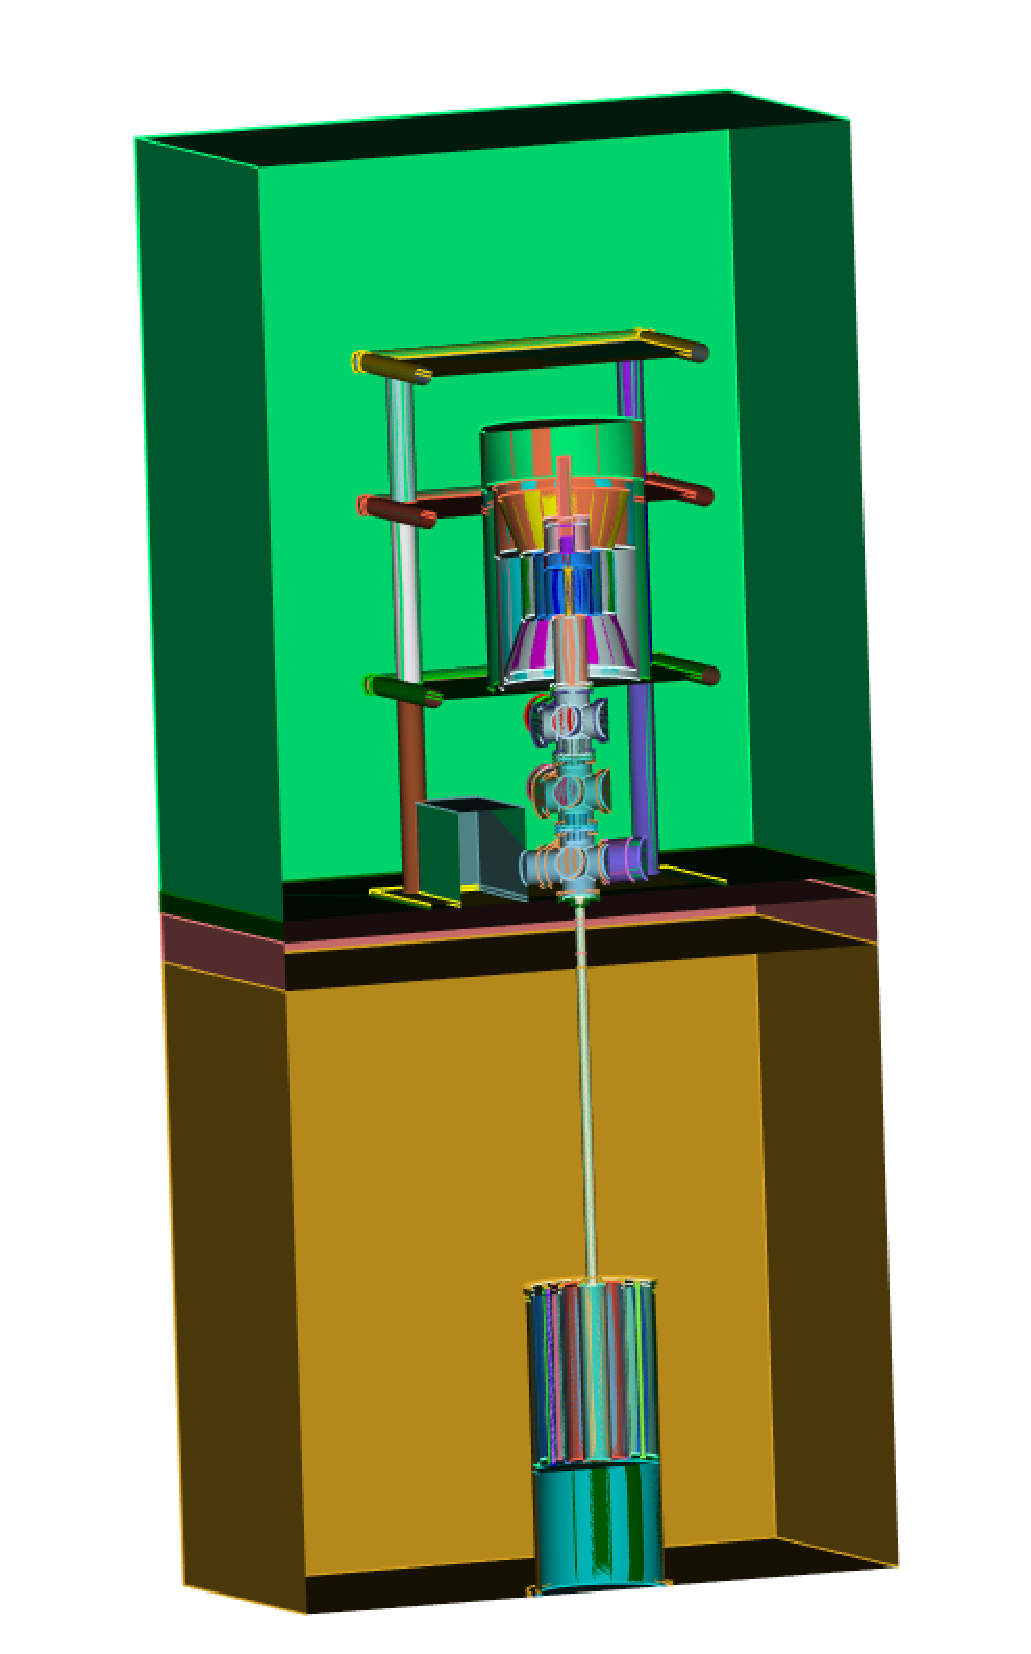
\includegraphics[width=0.4\textwidth]{SHINE.eps}
\caption{A cutaway view of the SHINE model used for demonstration of the SDF
  data structure.}
\label{fig:shine_sdf}
\end{figure}

A signed distance field with a 0.1 cm step size was applied to volumes near the
bottom of the model which contain both an aqueous solution of uraniaum sulfate
and a surounding light water moderator. As outlined in Table
\ref{tab:shine_sdf_result}, the resulting improvement in performance for a
simulation of 500,000 particles was approximately 35\% of the total runtime.

\begin{table}[H]
\centering
\begin{tabular}{c c c}
  \toprule
  \textbf{Implementation} & \textbf{Runtime (min)} & \textbf{Timing Ratio} \\
  \hline
  DAG-MCNP                & 76.14                  & 1.00                  \\
  DAG-MCNP w/ SDF         & 49.28                  & 0.65                  \\
  \bottomrule
\end{tabular}
\caption{Timing results for 500k particle histories of the SDF demonstration on
  the SHINE medical isotope production model.}
\label{tab:shine_sdf_result}
\end{table}

\section{Performance Mitigating Factors}\label{sec:sdf_limitations}

In the majority of the production models to which SDF geometry query
preconditioning was applied, the effect on the overall performance of the
simulation is much smaller than what was seen in the simple test cases. This is
due to a variety of factors, each of which is demonstrated by one of the models
in that table.

\subsection{Physics Dominant Simulations}\label{subsec:sdf_phys_dominant}

The nTOF model was selected as a charged particle transport demonstration. The
SDF was expected to be extremely beneficial in this scenario due to the high
collision density of charged particle transport relative to the size of certain
volumes in the problem. The computational time spent on the detailed of these
charged particles physics tends to dominate the runtime of the simulation,
leaving little room for improvement in the overall simulation runtime by
reducing geometric query costs.

As a neutral particle example of this occurs in SHINE as well. In order to
reduce the amount of time spend in the MCNP kernel for this calculation,
group-wise cross-sections were specified for all materials in the problem. This
allowed the SDF to have a more significant impact on the simulation runtime, but
may not be desirable if continuous energy cross sections are necessary for a
higher fidelity result.

\subsection{Utilization Model Assumptions}\label{subsec:sdf_util_model_limits}

There are some cases in which the SDF utilization model is inaccurate. The
calculation of the average chord length and average track length are assumed to
be true over the entirety of the volume in question. In reality, these values
will vary throughout the volume's domain. In cases where the local value of the
average chord length is smaller than predicted, the utilization model will overestimate
the SDF utilization. An example of this was found in the SNS test model.

A volume representing the mercury manifold in the SNS model was identified as a
good candidate for SDF application. The SDF analysis model estimates the
utilization of the SDF data structure under the assumption that the distribution
of particle interactions in the volume is uniform. In this case, particle
interactions occur mostly in regions of the volume where the local average chord
length is smaller than the average chord length of the entire volume. This
reduces the effectiveness of the SDF for the step size suggested by the input
script. Additionally, an SDF which would provide better utilization would
require a prohibitively small mesh step size in terms of the memory usage of the
data structure. These factors mean that this volume and in turn the SNS
simulation itself doesn't make it a candidate for application of the SDF as a
geometry query preconditioner.

\begin{sidewaysfigure}[h]
  \centering
  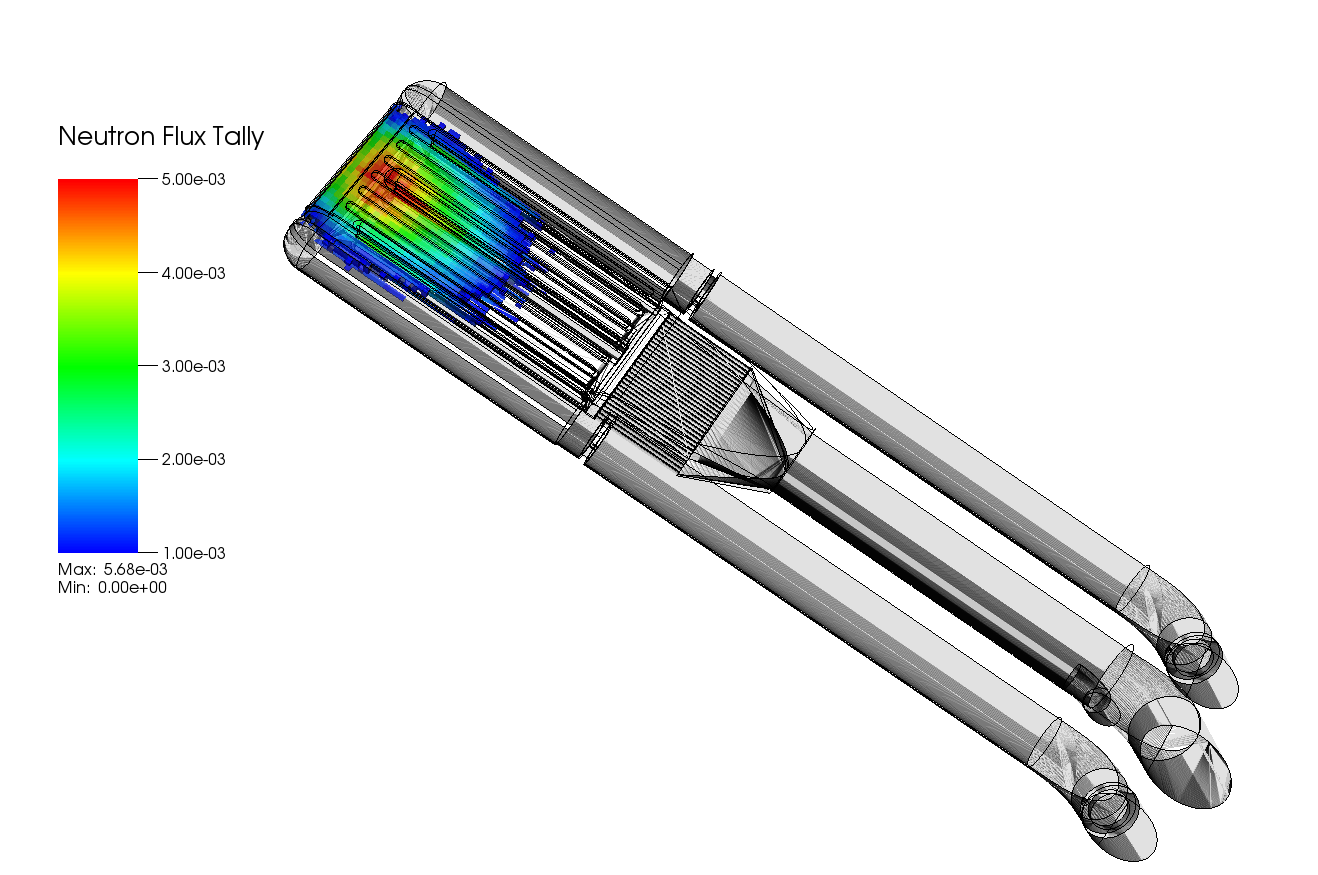
\includegraphics[width=\textwidth]{sns_vol16_flux.png}
  \caption{Example of utilization model limitation due to a small local average chord length
    in the region of high collition density.}
  \label{fig:sns_low_util}
\end{sidewaysfigure}

\subsection{Surface Mesh Complexity}\label{subsec:sdf_tree_depth}

In Section \ref{subsec:sdf_phys_dominant} limitations of the SDF impact on the
nTOF simulations were cited as related to the time spent in physics subroutines,
but the faceting of the particular volume which the SDF was applied to may play
a role as well. The volume's faceting contained a relatively small number of
triangles. This in turn means that the generated BVH for this volume was
relatively shallow. The relative improvement in performance when avoiding a ray
traversal is directly related to this tree depth. While the complexity of a BVH
search is $O(log\, N_{tri})$, the cost relative to the $O(1)$ look-up of a signed
distance value in the SDF becomes small as N becomes small, limiting the
effectiveness of the SDF regardless of the utilization.
